\documentclass[a4paper,12pt,titlepage]{article}
\usepackage{amsmath} 
\usepackage{amssymb}
\usepackage[nottoc]{tocbibind}
\usepackage{float}
\usepackage{indentfirst}
\author{\textit{Jiang Yicheng}\\\textit{515370910224}}
\title{\textbf{VV286\\ Honors Mathematics IV\\
Ordinary Differential Equations\\
		Assignment 9}}
\date{\today}
\usepackage{extarrows}
\usepackage{mathrsfs}
\usepackage{dsfont}
\usepackage[top=1in, bottom=1 in, left= 1in, right=1 in]{geometry}
\usepackage{fancyhdr,lastpage}
	\pagestyle{fancy}
	\fancyhf{}
\cfoot{Page \thepage\ of \pageref{LastPage}}
\usepackage{multirow}
\usepackage{gauss}
\usepackage{geometry}
\usepackage{graphicx}
\begin{document}

\maketitle

\section*{Exercise 9.1}
Set $y(x)=x^r\sum\limits_{k=0}^{\infty}a_kx^k$, since 
$$x^2y''+xy'+(x^2-9/4)y=0$$
then we can obtain that
\begin{align*}
\left\{
\begin{aligned}
&(r^2-9/4)a_0=0\\
&((r+1)^2-9/4)a_1=0\\
&((k+r+2)^2-9/4)a_{k+2}=-a_k,k\geqslant2\\
\end{aligned}
\right.\Leftrightarrow\left\{
\begin{aligned}
&r=3/2\vee r=-3/2\\
&a_1=0\\
&((k+r+2)^2-9/4)a_{k+2}=-a_k,k\geqslant0\\
\end{aligned}
\right.
\end{align*}
For $r=3/2$, we get one solution to the Bessel equation
$$x^2y''+xy'+(x^2-9/4)y=0$$
is
$$J_{3/2}=\sum\limits_{n=0}^{\infty}\dfrac{(-1)^n}{n!\Gamma(1+n+3/2)}\Big(\dfrac{x}{2}\Big)^{2n+3/2}$$

For $r=-3/2$, 
\begin{align*}
a_{2k+1}&=0,k\in\mathbb{N}\\
a_{2k}=&-\dfrac{1}{(2k)(2k-3)}a_{2k-2}=-\Big(\dfrac{1}{2}\Big)^2\dfrac{1}{k(k-3/2)}a_{2k-2}\\
=&\Big(\dfrac{1}{2}\Big)^{2k}\dfrac{(-1)^k}{k!\prod\limits_{i=1}^k(i-3/2)}a_0,k\in\mathbb{N}^*
\end{align*}
we can set $a_0=\dfrac{2^{3/2}}{\Gamma(-3/2)}=\dfrac{2^{3/2}(1-3/2)}{\Gamma(2-3/2)}$, then 
$$a_{2k}=\Big(\dfrac{1}{2}\Big)^{2k}\dfrac{(-1)^k}{k!\prod\limits_{i=1}^k(i-3/2)}\dfrac{2^{3/2}(1-3/2)}{\Gamma(2-3/2)}=\Big(\dfrac{1}{2}\Big)^{2k-3/2}\dfrac{(-1)^k}{k!\Gamma(1+k-3/2)}$$
this is also hold for $k=0$. So one solution is
$$J_{-3/2}(x)=x^{r}\sum\limits_{k=0}^{\infty}a_{k}x^k=\sum\limits_{n=0}^{\infty}\dfrac{(-1)^n}{n!\Gamma(1+n-3/2)}\Big(\dfrac{x}{2}\Big)^{2n-3/2}$$
So two independent solutions to the Bessel equation
$$x^2y''+xy'+(x^2-9/4)y=0$$
are
$$J_{3/2}(x)=\sum\limits_{n=0}^{\infty}\dfrac{(-1)^n}{n!\Gamma(1+n+3/2)}\Big(\dfrac{x}{2}\Big)^{2n+3/2}$$
$$J_{-3/2}(x)=\sum\limits_{n=0}^{\infty}\dfrac{(-1)^n}{n!\Gamma(1+n-3/2)}\Big(\dfrac{x}{2}\Big)^{2n-3/2}$$

\section*{Exercise 9.2}
\subsection*{i)}
Since
\begin{align*}
f(2m,2n):=&\int_0^{\pi}\cos^{2m}\theta\sin^{2n}\theta d\theta\\
=&-\dfrac{1}{2m+1}\int_0^{\pi}\sin^{2n-1}\theta d(\cos^{2m+1}\theta)\\
=&-\dfrac{1}{2m+1}(\sin^{2n-1}\theta \cos^{2m+1}\theta|_0^{\pi}-\int_0^{\pi}\cos^{2m+1}\theta d(\sin^{2n-1}\theta))\\
=&\dfrac{2n-1}{2m+1}\int_0^{\pi}\cos^{2m+2}\theta\sin^{2n-2}\theta d\theta\\
=&\dfrac{2n-1}{2m+1}\int_0^{\pi}\cos^{2m}\theta(1-\sin^2\theta)\sin^{2n-2}\theta d\theta\\
=&\dfrac{2n-1}{2m+1}(f(2m,2(n-1))-f(2m,2n))
\end{align*}
then we can get that
\begin{align*}
f(2m,2n)=\dfrac{2n-1}{2m+2n}f(2m,2(n-1))=\dfrac{\prod\limits_{i=1}^n(2i-1)}{\prod\limits_{i=1}^n(2m+2i)}f(2m,0)
\end{align*}
Also since
\begin{align*}
f(2m,0)=&\int_0^{\pi}\cos^{2m}\theta\sin^{0}\theta d\theta\\
=&\int_0^{\pi}\cos^{2m-2}\theta(1-\sin^2\theta) d\theta\\
=&\int_0^{\pi}\cos^{2m-2}\theta d\theta+\dfrac{1}{2m-1}\int_0^{\pi}\sin\theta d(\cos^{2m-1}\theta)\\
=&f(2(m-1),0)+\dfrac{1}{2m-1}(\sin\theta\cos^{2m-1}\theta|_0^{\pi}-\int_0^{\pi}\cos^{2m}\theta d\theta)\\
=&f(2(m-1),0)-\dfrac{1}{2m-1}f(2m,0)
\end{align*}
then
\begin{align*}
f(2m,0)=\dfrac{2m-1}{2m}f(2(m-1),0)=\dfrac{\prod\limits_{i=1}^m(2i-1)}{\prod\limits_{i=1}^m(2i)}f(0,0)=\dfrac{\prod\limits_{i=1}^m(2i-1)}{\prod\limits_{i=1}^m(2i)}\pi
\end{align*}
So
\begin{align*}
&\int_0^{\pi}\cos^{2m}\theta\sin^{2n}\theta d\theta\\
=&\dfrac{\prod\limits_{i=1}^n(2i-1)}{\prod\limits_{i=1}^n(2m+2i)}\dfrac{\prod\limits_{i=1}^m(2i-1)}{\prod\limits_{i=1}^m(2i)}\pi=\dfrac{(2n!)(2m)!}{2^{m+n}(m+n)!}\dfrac{1}{\prod\limits_{i=1}^m(2i)\prod\limits_{i=1}^n(2i)}\pi\\
=&\dfrac{(2n!)(2m)!}{2^{m+n}(m+n)!}\dfrac{1}{(2^mm!)(2^nn!)}\pi\\
=&\dfrac{(2m)!}{2^{2m}m!}\dfrac{(2n)!}{2^{2n}n!}\dfrac{\pi}{(m+n)!}
\end{align*}
To sum up
$$\int_0^{\pi}\cos^{2m}\theta\sin^{2n}\theta d\theta=\dfrac{(2m)!}{2^{2m}m!}\dfrac{(2n)!}{2^{2n}n!}\dfrac{\pi}{(m+n)!}
$$
\subsection*{ii)}
Since
$$\cos(x\cos\theta)=\sum\limits_{k=0}^{\infty}\dfrac{(-1)^k}{(2k)!}(x\cos\theta)^{2k}$$

\begin{align*}
&\dfrac{(2x)^nn!}{\pi(2n)!}\int_0^{\pi}\cos(x\cos\theta)\sin^{2n}\theta d\theta\\
=&\dfrac{(2x)^nn!}{\pi(2n)!}\int_0^{\pi}\sum\limits_{k=0}^{\infty}\dfrac{(-1)^k}{(2k)!}(x\cos\theta)^{2k}\sin^{2n}\theta d\theta=\dfrac{(2x)^nn!}{\pi(2n)!}\sum\limits_{k=0}^{\infty}\dfrac{(-1)^kx^{2k}}{(2k)!}\int_0^{\pi}(\cos\theta)^{2k}\sin^{2n}\theta d\theta\\
=&\dfrac{(2x)^nn!}{\pi(2n)!}\sum\limits_{k=0}^{\infty}\dfrac{(-1)^kx^{2k}}{(2k)!}\dfrac{(2k)!}{2^{2k}k!}\dfrac{(2n)!}{2^{2n}n!}\dfrac{\pi}{(k+n)!}\\
=&\sum\limits_{k=0}^{\infty}\dfrac{(-1)^k}{k!\Gamma(k+n+1)}\Big(\dfrac{x}{2}\Big)^{2k+n}\\
=&J_n(x)
\end{align*}
So
$$J_n(x)=\dfrac{(2x)^nn!}{\pi(2n)!}\int_0^{\pi}\cos(x\cos\theta)\sin^{2n}\theta d\theta$$

\subsection*{iii)}
Since
\begin{align*}
\int_0^{\pi}\sin(x\cos\theta)\sin^{2n}\theta d\theta
&=\int_0^{\frac{\pi}{2}}\sin(x\cos\theta)\sin^{2n}\theta d\theta+\int^{\pi}_{\frac{\pi}{2}}\sin(x\cos\theta)\sin^{2n}\theta d\theta\\
&=\int_0^{\frac{\pi}{2}}\sin(x\cos\theta)\sin^{2n}\theta d\theta+\int^{0}_{\frac{\pi}{2}}\sin(x\cos t)\sin^{2n}t dt\\
&=0
\end{align*}
then
\begin{align*}
&\dfrac{(2x)^nn!}{\pi(2n)!}\int_0^{\pi}e^{i(x\cos\theta)}\sin^{2n}\theta d\theta\\
=&\dfrac{(2x)^nn!}{\pi(2n)!}\int_0^{\pi}cos(x\cos\theta)\sin^{2n}\theta d\theta+i\dfrac{(2x)^nn!}{\pi(2n)!}\int_0^{\pi}sin(x\cos\theta)\sin^{2n}\theta d\theta\\
=&J_n(x)+0
\end{align*}

To sum up,
$$J_n(x)=\dfrac{(2x)^nn!}{\pi(2n)!}\int_0^{\pi}e^{i(x\cos\theta)}\sin^{2n}\theta d\theta$$

\subsection*{iv)}
Set $\xi=\cos\theta$, then 
$$\dfrac{d\theta}{d\xi}=\dfrac{d\arccos\xi}{d\xi}=-\dfrac{1}{\sqrt{1-\xi^2}}$$
So
\begin{align*}
J_n(x)&=\dfrac{(2x)^nn!}{\pi(2n)!}\int_0^{\pi}e^{i(x\cos\theta)}\sin^{2n}\theta d\theta=\dfrac{(2x)^nn!}{\pi(2n)!}\int_1^{-1}e^{i(x\xi)}(1-\xi^2)^n (-\dfrac{d\xi}{\sqrt{1-\xi^2}})\\
&=\dfrac{(2x)^nn!}{\pi(2n)!}\int_{-1}^{1}e^{i(x\xi)}(1-\xi^2)^{n-1/2} d\xi
\end{align*}
\section*{Exercise 9.3}
In this section, $\forall \nu\in\mathbb{R}\setminus\mathbb{Z}^-$,we denote
$$J_{\nu}(x)=\sum\limits_{k=0}^{\infty}\dfrac{(-1)^k}{k!\Gamma(k+\nu+1)}\Big(\dfrac{x}{2}\Big)^{2k+\nu}$$
$\forall \nu\in\mathbb{Z}^-$ we denote
$$J_{\nu}(x)=(-1)^{\nu}J_{-\nu}(x)$$
\subsection*{i)}
$\forall\nu\in\mathbb{R}$
\begin{align*}
\dfrac{d}{dx}(x^{\nu}J_{\nu}(x))=&\dfrac{d}{dx}(x^{\nu}\sum\limits_{k=0}^{\infty}\dfrac{(-1)^k}{k!\Gamma(k+\nu+1)}\Big(\dfrac{x}{2}\Big)^{2k+\nu})\\
=&\sum\limits_{k=0}^{\infty}\dfrac{(-1)^k(2k+2\nu)}{k!(k+\nu)\Gamma(k+\nu)}\Big(\dfrac{x}{2}\Big)^{2k+2\nu-1}\cdot\dfrac{1}{2})\\
=&x^{\nu}\sum\limits_{k=0}^{\infty}\dfrac{(-1)^k}{k!\Gamma(k+\nu-1+1)}\Big(\dfrac{x}{2}\Big)^{2k+\nu-1}\\
=&x^{\nu}J_{\nu-1}
\end{align*}
So $\dfrac{d}{dx}(x^{\nu}J_{\nu}(x))=x^{\nu}J_{\nu-1}$

\subsection*{ii)}
$\forall\nu\in\mathbb{R}$
\begin{align*}
\dfrac{d}{dx}(x^{-\nu}J_{\nu}(x))=&\dfrac{d}{dx}(x^{-\nu}\sum\limits_{k=0}^{\infty}\dfrac{(-1)^k}{k!\Gamma(k+\nu+1)}\Big(\dfrac{x}{2}\Big)^{2k+\nu})\\
=&\sum\limits_{k=1}^{\infty}\dfrac{(-1)^k(2k)}{k!\Gamma(k+\nu+1)}\Big(\dfrac{x}{2}\Big)^{2k-1}\cdot\dfrac{1}{2})\\
=&x^{-\nu}\sum\limits_{k=0}^{\infty}\dfrac{(-1)^{k+1}}{k!\Gamma(k+(\nu+1)+1)}\Big(\dfrac{x}{2}\Big)^{2k+\nu+1}\\
=&x^{-\nu}J_{\nu+1}
\end{align*}
So $\dfrac{d}{dx}(x^{-\nu}J_{\nu}(x))=x^{-\nu}J_{\nu+1}$

\subsection*{iii)}
\begin{align*}
&2\nu J_{\nu}(x)-xJ_{\nu+1}(x)-xJ_{\nu-1}(x)\\
=&2\nu\sum\limits_{k=0}^{\infty}\dfrac{(-1)^k}{k!\Gamma(k+\nu+1)}\Big(\dfrac{x}{2}\Big)^{2k+\nu}-x\sum\limits_{k=0}^{\infty}\dfrac{(-1)^k}{k!\Gamma(k+\nu+1+1)}\Big(\dfrac{x}{2}\Big)^{2k+\nu+1}\\
&-x\sum\limits_{k=0}^{\infty}\dfrac{(-1)^k}{k!\Gamma(k+\nu-1+1)}\Big(\dfrac{x}{2}\Big)^{2k+\nu-1}\\
=&2\nu\sum\limits_{k=0}^{\infty}\dfrac{(-1)^k}{k!\Gamma(k+\nu+1)}\Big(\dfrac{x}{2}\Big)^{2k+\nu}-2\sum\limits_{k=0}^{\infty}\dfrac{(-1)^k}{k!\Gamma(k+1+\nu+1)}\Big(\dfrac{x}{2}\Big)^{2(k+1)+\nu}\\
&-2\sum\limits_{k=0}^{\infty}\dfrac{(-1)^k}{k!\Gamma(k+\nu)}\Big(\dfrac{x}{2}\Big)^{2k+\nu}\\
=&2\nu\sum\limits_{k=0}^{\infty}\dfrac{(-1)^k}{k!\Gamma(k+\nu+1)}\Big(\dfrac{x}{2}\Big)^{2k+\nu}+2\sum\limits_{k=0}^{\infty}\dfrac{(-1)^kk}{k!\Gamma(k+\nu+1)}\Big(\dfrac{x}{2}\Big)^{2k+\nu}\\
&-2\sum\limits_{k=0}^{\infty}\dfrac{(-1)^k}{k!\Gamma(k+\nu)}\Big(\dfrac{x}{2}\Big)^{2k+\nu}\\
=&2\sum\limits_{k=0}^{\infty}\dfrac{(-1)^k}{k!\Gamma(k+\nu)}\Big(\dfrac{x}{2}\Big)^{2k+\nu}-2\sum\limits_{k=0}^{\infty}\dfrac{(-1)^k}{k!\Gamma(k+\nu)}\Big(\dfrac{x}{2}\Big)^{2k+\nu}\\
=&0
\end{align*}
So $2\nu J_{\nu}(x)=xJ_{\nu+1}(x)+xJ_{\nu-1}(x)$

\subsection*{iv)}
\begin{align*}
&J'_{\nu}(x)\\
=&\dfrac{d}{dx}\sum\limits_{k=0}^{\infty}\dfrac{(-1)^k}{k!\Gamma(k+\nu+1)}\Big(\dfrac{x}{2}\Big)^{2k+\nu}\\
=&\dfrac{1}{2}\sum\limits_{k=0}^{\infty}\dfrac{(-1)^k(2k+\nu)}{k!\Gamma(k+\nu+1)}\Big(\dfrac{x}{2}\Big)^{2k+\nu-1}\\
=&\dfrac{1}{2}\sum\limits_{k=0}^{\infty}\dfrac{(-1)^k(k+\nu)}{k!\Gamma(k+\nu+1)}\Big(\dfrac{x}{2}\Big)^{2k+\nu-1}+\dfrac{1}{2}\sum\limits_{k=0}^{\infty}\dfrac{(-1)^kk}{k!\Gamma(k+\nu+1)}\Big(\dfrac{x}{2}\Big)^{2k+\nu-1}\\
=&\dfrac{1}{2}\sum\limits_{k=0}^{\infty}\dfrac{(-1)^k}{k!\Gamma(k+\nu-1+1)}\Big(\dfrac{x}{2}\Big)^{2k+\nu-1}+\dfrac{1}{2}\sum\limits_{k=1}^{\infty}\dfrac{(-1)^k}{(k-1)!\Gamma(k+\nu+1)}\Big(\dfrac{x}{2}\Big)^{2k+\nu-1}\\
=&\dfrac{1}{2}\sum\limits_{k=0}^{\infty}\dfrac{(-1)^k}{k!\Gamma(k+\nu-1+1)}\Big(\dfrac{x}{2}\Big)^{2k+\nu-1}+\dfrac{1}{2}\sum\limits_{k=1}^{\infty}\dfrac{(-1)^{k+1}}{k!\Gamma(k+\nu+1+1)}\Big(\dfrac{x}{2}\Big)^{2k+\nu+1}\\
=&\dfrac{1}{2}(J_{\nu-1}(x)-J_{\nu+1}(x))
\end{align*}
So $J'_{\nu}(x)=\dfrac{1}{2}(J_{\nu-1}(x)-J_{\nu+1}(x))$
 
\section*{Exercise 9.4}
For a suspended chain of constant density, the tension is given by
$$T(x) =\int\rho\cdot g \cdot dx=\int_0^x\rho_0\cdot g\cdot x^{\mu}=\rho_0g\dfrac{1}{\mu+1}x^{\mu+1}$$
from gravity and we have no additional external forces, so the model equation is
\begin{align*}
&\rho u_{tt}(x,t)=\dfrac{\partial}{\partial x}(Tu_x)\\
\Leftrightarrow &\rho_0\cdot x^{\mu}u_{tt}(x,t)=\rho_0\cdot g\cdot x^{\mu}u_{x}+\dfrac{1}{\mu+1}\rho_0\cdot g\cdot x^{\mu+1}u_{xx}\\
\Leftrightarrow &\dfrac{\mu+1}{g}u_{tt}(x,t)=(\mu+1)u_x+xu_{xx}
\end{align*}
Set $u(x,t)=y(x)\cdot e^{i\omega t}$, then
\begin{align*}
\dfrac{(\mu+1)}{g}y(x)\cdot(-\omega^2e^{i\omega t})=(\mu+1)y'(x)\cdot e^{i\omega t}+x\cdot y''(x)e^{i\omega t}
\end{align*}
Set $f(z)=x^{\mu/2}y(x),x=gz^2/(4(\mu+1)\omega^2)$, so $y(x)=\Big(\dfrac{gz^2}{4(\mu+1)\omega^2}\Big)^{-\mu/2}f(z)$, $z=2\sqrt{\mu+1}\omega\sqrt{x/g}$, then
\begin{align*}
y'(x)&=\dfrac{dy}{dz}\dfrac{dz}{dx}=\dfrac{\sqrt{\mu+1}\omega}{\sqrt{gx}}\Big(\dfrac{g}{4(\mu+1)\omega^2}\Big)^{-\mu/2}(-\mu z^{-\mu-1}f(z)+z^{-\mu}f'(z))\\
&=\dfrac{2(\mu+1)\omega^2}{g}\Big(\dfrac{g}{4(\mu+1)\omega^2}\Big)^{-\mu/2}(-\mu z^{-\mu-2}f(z)+z^{-\mu-1}f'(z))
\end{align*}
\begin{align*}
y''(x)=\dfrac{dy'(x)}{dz}\dfrac{dz}{dx}=&\dfrac{4(\mu+1)^2\omega^4}{zg^2}\Big(\dfrac{g}{4(\mu+1)\omega^2}\Big)^{-\mu/2}\\
&\cdot(\mu(\mu+2)z^{-\mu-3}f(z)-(2\mu+1)z^{-\mu-2}f'(z)+z^{-\mu-1}f''(z))
\end{align*}
Since $xy''(x)+(\mu+1)y'(x)+\dfrac{(\mu+1)\omega^2}{g}y(x)=0$, we get that
\begin{align*}
0=&\dfrac{gz^2}{4(\mu+1)\omega^2}\dfrac{4(\mu+1)^2\omega^4}{zg^2}\Big(\dfrac{g}{4(\mu+1)\omega^2}\Big)^{-\mu/2}\\
&\cdot(\mu(\mu+2)z^{-\mu-3}f(z)-(2\mu+1)z^{-\mu-2}f'(z)+z^{-\mu-1}f''(z))\\
&+(\mu+1)\dfrac{2(\mu+1)\omega^2}{g}\Big(\dfrac{g}{4(\mu+1)\omega^2}\Big)^{-\mu/2}(-\mu z^{-\mu-2}f(z)+z^{-\mu-1}f'(z))\\
&+\dfrac{(\mu+1)\omega^2}{g}\Big(\dfrac{gz^2}{4(\mu+1)\omega^2}\Big)^{-\mu/2}f(z)
\end{align*}
So
$$z^2f''(z)+zf'(z)+(z^2-\mu^2)f(z)=0$$
This is precisely the Bessel equation of order $\mu$, since we are looking for solutions that are finite at $x = 0$ (the end of the
chain), so we obtain
$$f(z)=c\cdot J_{\mu}(z)$$
Substituting back,
$$y(x)=-c\cdot x^{-\mu/2}\cdot J_{\mu}(2\sqrt{\mu+1}\omega\sqrt{x/g})$$
The boundary condition at the upper end implies
$$y(l)=0=-c\cdot x^{-\mu/2}\cdot J_{\mu}(2\sqrt{\mu+1}\omega\sqrt{x/g})$$
So we see that
$$\omega=\dfrac{1}{2\sqrt{\mu+1}}\sqrt{\frac{g}{l}}\cdot\alpha_{\mu,n}$$
where $\alpha_{\mu,n}, n = 1, 2,\cdots$ is the $n^{th}$ zero of $J_{\mu}$, the Bessel function of order $\mu$.

\section*{Exercise 9.5}
\subsection*{i)}
Since $u(x,t) = X(x)e^{i\omega t},\dfrac{T}{\rho}u_{xx}=u_{tt},u(0)=u(l)=0$
$$\dfrac{T}{\rho_0}X''(x)e^{i\omega t}=X(x)(-\omega^2)e^{i\omega t},X(0)=X(l)=0$$
i.e.
$$X''(x)=-\dfrac{\omega^2\rho_0}{T}X(x)$$
the genenral solution to it is
$$X(x)=A\cos(\sqrt{\dfrac{\omega^2\rho_0}{T}}x+\varphi)$$
so
$$0=X(0)=A\cos(\varphi),0=X(l)=A\cos(\sqrt{\dfrac{\omega^2\rho_0}{T}}l+\varphi)$$
so
$$\varphi=\dfrac{\pi}{2}+k_1\pi,\sqrt{\dfrac{\rho_0}{T}}\omega l+\varphi=\dfrac{\pi}{2}+k_2\pi,k_1,k_2\in\mathbb{Z}$$
so
$$\omega=\dfrac{k\pi}{l}\sqrt{\dfrac{T}{\rho_0}},k\in\mathbb{Z}$$
is the frequencies of the normal modes.
\subsection*{ii)}
Since $u(x,t) = X(x)e^{i\omega t},\dfrac{T}{\rho}u_{xx}=u_{tt},u(0)=u(l)=0$
$$\dfrac{T}{\rho_0\xi}X''(x)e^{i\omega t}=X(x)(-\omega^2)e^{i\omega t},X(0)=X(l)=0$$
so
$$X''(x)+\dfrac{\omega^2\rho_0\xi}{T}X(x)=0$$
since $\xi=1+\dfrac{kx}{l}$, set $Y(\xi)=X(x)$, then
$$Y'(\xi)=\dfrac{dX(x)}{dx}\dfrac{dx}{d\xi}=\dfrac{l}{k}X'(x),Y''(\xi)=\dfrac{dY'(\xi)}{dx}\dfrac{dx}{d\xi}=\dfrac{l^2}{k^2}X''(x)$$
So
$$Y''(\xi)+\dfrac{\rho_0\omega^2l^2}{k^2T}\xi Y(\xi)=\dfrac{l^2}{k^2}(X''(x)+\dfrac{\rho_0\omega^2}{T}\xi X(x))=0$$
Set $\kappa^2=\dfrac{\rho_0\omega^2l^2}{k^2T}$ then $Y''(\xi)+\kappa^2\xi Y(\xi)=0$. Set $Z(t)=Y(\xi),t=\kappa^{2/3}\xi$, then
$$Y'(\xi)=\dfrac{dZ(t)}{dt}\dfrac{dt}{d\xi}=\kappa^{2/3}Z'(t),Y''(\xi)=\dfrac{dZ'(t)}{dt}\dfrac{dt}{d\xi}=\kappa^{4/3}Z''(t)$$
So
$$Z''(t)+tZ(t)=0$$
and the solution to this Airy equation 
\begin{align*}
Z(t)=t^{1/2}(c_1J_{1/3}(\dfrac{2}{3}t^{3/2})+c_2J_{-1/3}(\dfrac{2}{3}t^{3/2}))
\end{align*}
So
\begin{align*}
Y(\xi)=&Z(t)=(\kappa^{2/3}\xi)^{1/2}(c_1J_{1/3}(\dfrac{2}{3}(\kappa^{2/3}\xi)^{3/2})+c_2J_{-1/3}(\dfrac{2}{3}(\kappa^{2/3}\xi)^{3/2}))\\
=&\kappa^{1/3}\xi^{1/2}(c_1J_{1/3}(\dfrac{2}{3}\kappa\xi^{3/2})+c_2J_{-1/3}(\dfrac{2}{3}\kappa\xi^{3/2}))
\end{align*}
So
\begin{align*}
X(x)=&Y(\xi)=\kappa^{1/3}(1+\dfrac{kx}{l})^{1/2}(c_1J_{1/3}(\dfrac{2}{3}\kappa(1+\dfrac{kx}{l})^{3/2})+c_2J_{-1/3}(\dfrac{2}{3}\kappa(1+\dfrac{kx}{l})^{3/2}))
\end{align*}
Since $X(0)=X(l)=0$, we obtain that
\begin{align*}
\left\{
\begin{aligned}
&c_1J_{1/3}(\dfrac{2}{3}\kappa)+c_2J_{-1/3}(\dfrac{2}{3}\kappa)=0\\
&c_1J_{1/3}(\dfrac{2}{3}\kappa(1+k)^{3/2})+c_2J_{-1/3}(\dfrac{2}{3}\kappa(1+k)^{3/2})=0\\
\end{aligned}
\right.
\end{align*}
To get non-trival solution for $c_1,c_2$, 
$$J_{1/3}(\dfrac{2}{3}\kappa)J_{-1/3}(\dfrac{2}{3}\kappa(1+k)^{3/2})=J_{-1/3}(\dfrac{2}{3}\kappa)J_{1/3}(\dfrac{2}{3}\kappa(1+k)^{3/2})$$
Denote $\mu=\dfrac{2}{3}\kappa$ is the solution to the equation 
$$J_{1/3}(\mu)J_{-1/3}(\mu(1+k)^{3/2})=J_{-1/3}(\mu)J_{1/3}(\mu(1+k)^{3/2})$$
Then
$$\dfrac{9}{4}\mu^2=\kappa^2=\dfrac{\rho_0\omega^2l^2}{k^2T}$$
So
$$\omega^2=\dfrac{9\mu^2k^2T}{4\rho_0l^2}$$

\section*{Exercise 9.6}
In the lecture we have seen that
$$l_{max}=\sqrt[3]{\dfrac{9\alpha_{-1/3,1}^2EI}{4q}}$$
Use mathematica we find that $\alpha_{-1/3,1}=1.86635$.
\begin{figure}[H]
    \centering
    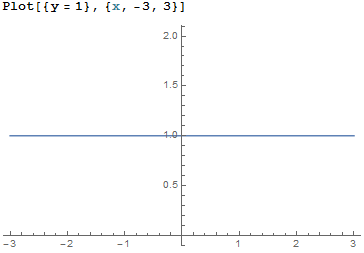
\includegraphics[scale=1]{1.png}
\end{figure}
From wikipedia, we find $E_{steel}=200\times10^9Pa$, also we know that for a hollow pole with inner radius $r$ and outer radius $0.1m$ its moment of inertia is
$$I=\dfrac{1}{2}m(r^2+0.01)=\dfrac{1}{2}\rho\pi(0.01-r^2)l_{max}(r^2+0.01)$$
and its uniform load is
$$q=\dfrac{mg}{l}=g\rho\pi(0.01-r^2)$$
So
$$l_{max}=\sqrt[3]{\dfrac{9\alpha_{-1/3,1}^2El_{max}(r^2+0.01)}{8g}}\Rightarrow l_{max}=\sqrt{\dfrac{9\cdot 1.86635^2\cdot 200\times 10^9\times 0.01\times2}{8\times9.80665}}=39980m$$
So the maximum height to which I can build the flagpole is 39980m.


\section*{Exercise 9.7}

\subsection*{i)}
For $x>0$, since $\Gamma(x+1)=x\Gamma(x)$, then
$$\Gamma'(x+1)=\dfrac{d\Gamma(x+1)}{dx}=\dfrac{dx\Gamma(x)}{dx}=\Gamma(x)+x\Gamma'(x)$$
So
$$\psi(x+1)=\dfrac{\Gamma'(x+1)}{\Gamma(x+1)}=\dfrac{\Gamma(x)+x\Gamma'(x)}{x\Gamma(x)}=\dfrac{1}{x}+\psi(x)$$
i.e.
$$\psi(x+1)=\dfrac{1}{x}+\psi(x)$$

\subsection*{ii)}
Since $\psi(x+1)=\dfrac{1}{x}+\psi(x)$,
\begin{align*}
\psi(n+1)=\dfrac{1}{n}+\psi(n)=\psi(1)+\sum\limits_{k=1}^n\dfrac{1}{k}
\end{align*}
Since 
$$\psi(1)=\dfrac{\Gamma'(1)}{\Gamma(1)}=\dfrac{-\gamma}{\int_0^{\infty}e^{-y}dy}=\dfrac{-\gamma}{-e^{-y}|_0^{\infty}}=-\gamma$$
So
$$\psi(n+1)=-\gamma+\sum\limits_{k=1}^n\dfrac{1}{k}$$

\subsection*{iii)}
According to Stirling's formula, $n!\sim \sqrt{2\pi n}\Big(\dfrac{n}{e}\Big)^n$, also we know that $\Gamma(n+1)=n!$, so
$\Gamma(x+1)\sim \sqrt{2\pi x}\Big(\dfrac{x}{e}\Big)^x$ as $x\rightarrow \infty$. So
\begin{align*}
\Gamma'(x+1)&=\sqrt{\dfrac{\pi}{2x}}\Big(\dfrac{x}{e}\Big)^x+\sqrt{2\pi x}(-e^{-x}x^x+e^{-x}x^x(\ln x+1))
\end{align*}
So as $x\rightarrow\infty$
\begin{align*}
\psi(x+1)=\dfrac{\Gamma'(x+1)}{\Gamma(x+1)}=\dfrac{\sqrt{2\pi x}\Big(\dfrac{x}{e}\Big)^x(\dfrac{1}{2x}+\ln x)}{\sqrt{2\pi x}\Big(\dfrac{x}{e}\Big)^x}=\dfrac{1}{2x}+\ln x+O\Big(\dfrac{1}{x^2}\Big)
\end{align*}
So
$$-\gamma+\sum\limits_{k=1}^n\dfrac{1}{k}=\psi(n+1)=\ln(n)+\dfrac{1}{2n}+O\Big(\dfrac{1}{n^2}\Big)$$
i.e.
$$\sum\limits_{k=1}^n\dfrac{1}{k}=\gamma+\ln(n)+\dfrac{1}{2n}+O\Big(\dfrac{1}{n^2}\Big)$$
\section*{Exercise 9.8}
\subsection*{i)}

As $\nu\rightarrow0$, $J_{\nu}(x)\cos(\nu \pi)-J_{-\nu}(x)\rightarrow0,\sin(\nu \pi)\rightarrow0$, so we can use l'Hospital's rule,
\begin{align*}
Y_0(x)=&\underset{\nu\rightarrow0}{\lim}\dfrac{J_{\nu}(x)\cos(\nu \pi)-J_{-\nu}(x)}{\sin(\nu \pi)}\\
=&\underset{\nu\rightarrow0}{\lim}\dfrac{J_{\nu}(x)(-\pi\sin(\nu \pi))+\frac{dJ_{\nu}(x)}{d\nu}\cos(\nu\pi)-\frac{dJ_{-\nu}(x)}{d\nu}}{\pi\cos(\nu \pi)}\\
=&\underset{\nu\rightarrow0}{\lim}\dfrac{J_{\nu}(x)(-\pi\sin(\nu \pi))+\frac{dJ_{t}(x)}{dt}|_{t=\nu}\cos(\nu\pi)+\frac{dJ_{t}(x)}{dt}|_{t=-\nu}}{\pi\cos(\nu \pi)}\\
=&\dfrac{1}{\pi}(\frac{dJ_{t}(x)}{dt}|_{t=0}+\frac{dJ_{t}(x)}{dt}|_{t=0})\\
=&\dfrac{2}{\pi}\frac{dJ_{\nu}(x)}{d\nu}|_{\nu=0}
\end{align*}
So $Y_0(x)=\dfrac{2}{\pi}\dfrac{dJ_{\nu}(x)}{d\nu}|_{\nu=0}$.
\subsection*{ii)}
\begin{align*}
Y_0(x)=&\dfrac{2}{\pi}\dfrac{dJ_{\nu}(x)}{d\nu}\Big|_{\nu=0}=Y_0(x)=\dfrac{2}{\pi}\dfrac{d}{d\nu}\sum\limits_{k=0}^{\infty}\dfrac{(-1)^k}{k!\Gamma(k+\nu+1)}\Big(\dfrac{x}{2}\Big)^{2k+\nu}\Big|_{\nu=0}\\
=&\dfrac{2}{\pi}\Big(\sum\limits_{k=0}^{\infty}\dfrac{(-1)^k(-\Gamma'(k+\nu+1))}{k!(\Gamma(k+\nu+1))^2}\Big(\dfrac{x}{2}\Big)^{2k+\nu}\Big|_{\nu=0}+\sum\limits_{k=0}^{\infty}\dfrac{(-1)^k}{k!\Gamma(k+\nu+1)}\Big(\dfrac{x}{2}\Big)^{2k+\nu}\ln(\dfrac{x}{2})\Big|_{\nu=0}\Big)\\
=&\dfrac{2}{\pi}\Big(-\sum\limits_{k=0}^{\infty}\dfrac{(-1)^k(\psi(k+\nu+1))}{k!\Gamma(k+\nu+1)}\Big(\dfrac{x}{2}\Big)^{2k+\nu}\Big|_{\nu=0}+J_0(x)\ln(\dfrac{x}{2})\Big)\\
=&\dfrac{2}{\pi}\Big(-\sum\limits_{k=0}^{\infty}\dfrac{(-1)^k(\psi(k+1))}{k!\Gamma(k+1)}\Big(\dfrac{x}{2}\Big)^{2k}+J_0(x)\ln(\dfrac{x}{2})\Big)\\
=&\dfrac{2}{\pi}\Big(-\sum\limits_{k=0}^{\infty}\dfrac{(-1)^k(-\gamma+\sum\limits_{k=1}^n\dfrac{1}{k})}{k!\Gamma(k+1)}\Big(\dfrac{x}{2}\Big)^{2k}+J_0(x)\ln(\dfrac{x}{2})\Big)\\
=&\dfrac{2}{\pi}\Big(-\sum\limits_{k=0}^{\infty}\dfrac{(-1)^k\sum\limits_{k=1}^n\dfrac{1}{k}}{(k!)^2}\Big(\dfrac{x}{2}\Big)^{2k}+J_0(x)\ln(\dfrac{x}{2})+\gamma J_0(x)\Big)\\
=&\dfrac{2}{\pi}J_0(x)\Big(\ln\Big(\dfrac{x}{2}\Big)+\gamma\Big)-\dfrac{2}{\pi}\sum\limits_{k=0}^{\infty}\dfrac{(-1)^k\sum\limits_{k=1}^n\dfrac{1}{k}}{(k!)^2}\Big(\dfrac{x}{2}\Big)^{2k}
\end{align*}
So
$$Y_0(x)=\dfrac{2}{\pi}J_0(x)\Big(\ln\Big(\dfrac{x}{2}\Big)+\gamma\Big)-\dfrac{2}{\pi}\sum\limits_{n=0}^{\infty}\dfrac{(-1)^n}{(n!)^2}\Big(\dfrac{x}{2}\Big)^{2n}H_n$$
where $H_n=1+1/2+1/3+\cdots+1/n$








\end{document}
